\section{Arduinoen og programmering} \label{sec:arduino}
%--------------- Indsæt en arduino ---------------%
\begin{figure}[H]
	\centering
    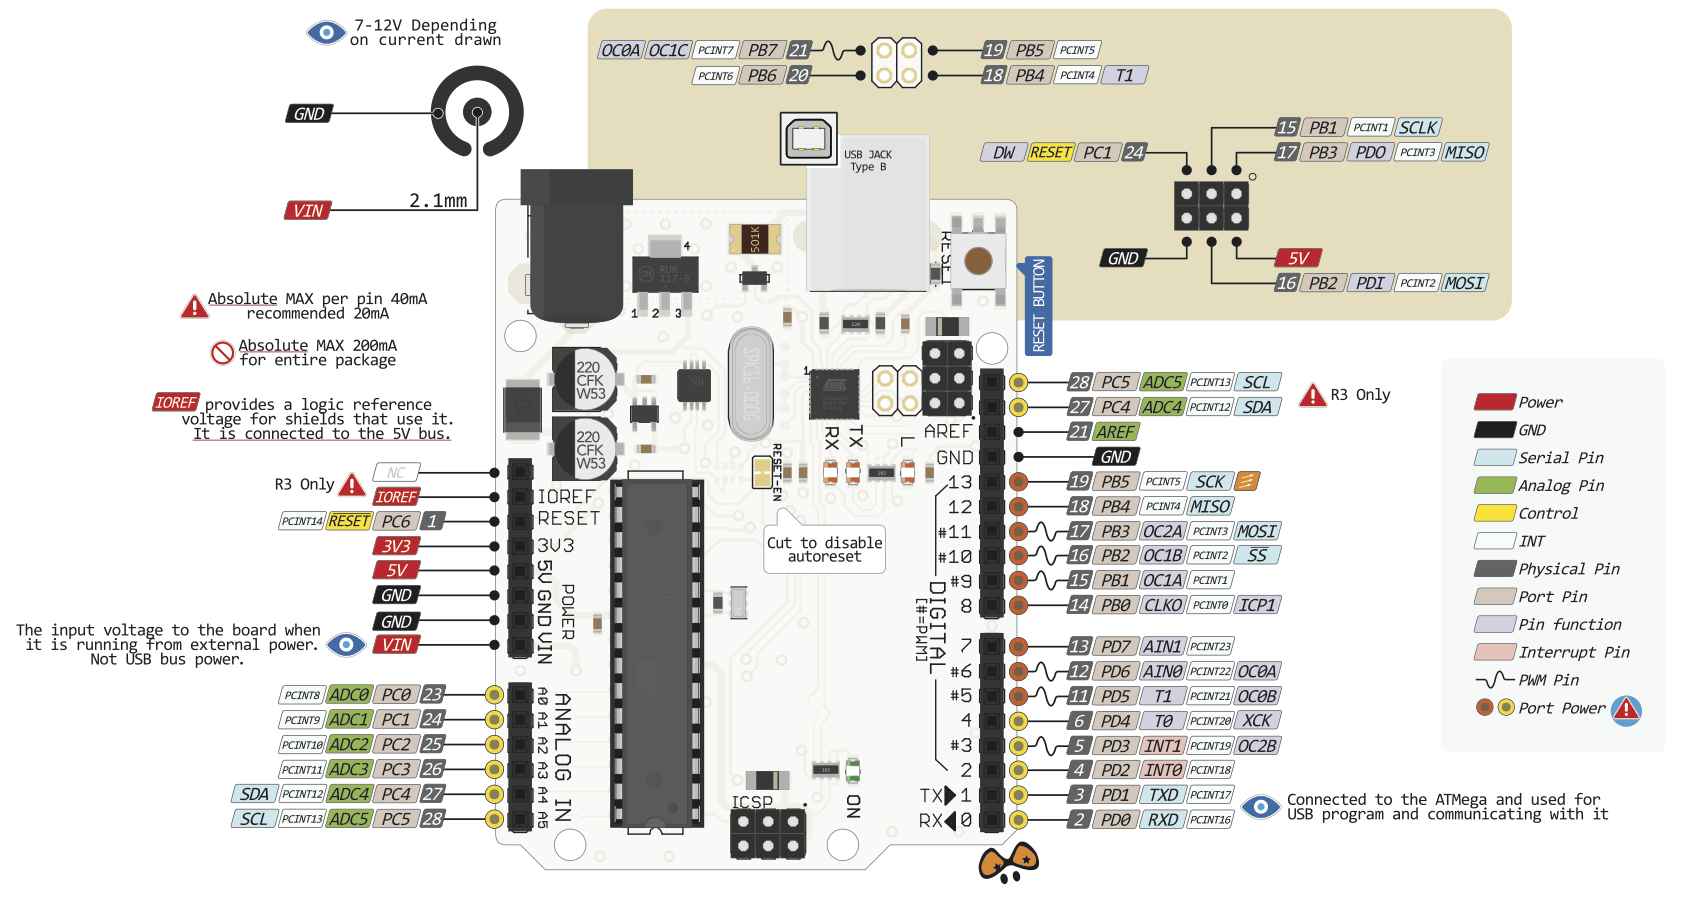
\includegraphics[width=\textwidth]{figures/arduino/portmani.PNG}
	\caption{Arduino uno med ATmega328}
	\label{fig:portmani}
	Her kan man se hvilke ben der er på Arduinoen, og hvilke porte de fordelt på ( PORTB, PORTC og PORTD). Hvis man ser på "Port pin", står der P for port, efterfulgt af bogstavet for hvilken port den er tildelt, efterfulgt af dens bit position i den port.\\
	Vi har også opgivet den påkrævede spænding for at køre Arduinoen. Vi kan også se Analog input ben (A0-A5) og de digital input og output ben (0-13). Vi kan se ud fra analog ben A4 og A5 at de er SDA og SCL, som er relevant når vi skal benytte I2C kredsen.
	\\Kilde: \url{http://pighixxx.com/unov3pdf.pdf}
\end{figure}
\subsection{Analog inputs og outputs (PWM)}\label{sec:ard:analog}
Analog input i Arduinoen er et input som beskriver spændingsfaldet over inputtet og jord med et 10 bit tal.\cite{arduinoAnalog} Dette betyder at den laveste værdi og højeste værdi af et analog input er
\begin{align}
\SI{}{U_{MIN}}&=b00\,0000\,0000\rightarrow 0\rightarrow \SI{0}{V}\\
\SI{}{U_{MAX}}&=b11\,1111\,1111\rightarrow 1023\rightarrow \SI{5}{V}\\
\end{align}
Med Arduinoen kan man få et analog input igennem en analog ben (se \ref{fig:portmani}), og kalde metoden \emph{analogRead()} til benets nummer, eksempelvis A0. Da vores precision er på 10 bit, til at beskrive et maks spændingsfald på $\SI{5}{V}$, må det gælde at den laveste ændring i spændingsfaldet vi kan måle er
\begin{align}
U_{prec}&=\frac{\SI{5}{V}}{1023}\approx \SI{5d-3}{V}
\end{align}
\subsection{Digital inputs og outputs}
\subsection{I2C - Synkroniseret kommunikation}


%-------------------------------------------------------------------------------------------------------------------------------------------
%--------------------------------------- PROGRAMMING PART ----------------------------------------------------------------------------------
%-------------------------------------------------------------------------------------------------------------------------------------------
\subsection{Kort beskrivelse af programmets formål}

Programmet til master Arduinoen \ref{bilag:programMaster} og Controller Arduinoen i bilag \ref{bilag:programController}, som er kommenteret. De mest komplekse og primære funktioner vi har programmeret, er beskrevet i sektion \ref{sec:primaerefunc}.
\subsection{Oversigt over inputs og outputs og lokation}
\begin{table}[H]
	\caption{Inputs og outputs for Master Arduinoen} % title
	\label{tab:IOMaster}
	\centering
		\begin{tabular}{c|c c} 
		Ben & I/O & Forbundet komponent\\ [0.5ex] 
		\hline 
			2 & Output & Stepper motor\\
			3 & Output & Stepper motor\\
			4 & Output & Stepper motor\\
			5 & Output & Stepper motor\\
			6 & Output & Trækmotor\\
			9 & Output & Gearmotor (fri)\\
			10 & Output & Gearmotor (lås)\\
			11 & Output & Ladningssensor LED (grøn)\\
			12 & Output & Ladningssensor LED (rød)\\
			13 & Output & Ladningssensor LED (blå)\\
			A0 & Input & Ladningssensor Fotodiode\\
			A1 & Input & Hastighedssensor 1\\			
			A2 & Input & Hastighedssensor 2\\
			A4 (SDA) & Output & I2C kommunikation\\
			A5 (SCL) & I/O & I2C kommunikation\\[1ex]
		\hline %inserts single line
	\end{tabular}
\end{table}

\begin{table}[H]
	\caption{Inputs og outputs for Controller Arduinoen} % title
	\label{tab:IOController}
	\centering
		\begin{tabular}{c|c c} 
		Ben & I/O & Forbundet komponent\\ [0.5ex] 
		\hline 
			2 & I/O & LCD (DB7)\\
			3 & I/O & LCD (DB6)\\
			4 &I/O & LCD (DB5)\\
			5 &I/O & LCD (DB4)\\
			11 & Output & LCD (E)\\
			12 &Output & LCD (RS)\\
			A0 & Input & Knap (ryg kanon op)\\
			A1 & Input & Knap (ryg kanon ned)\\			
			A2 & Input & Knap (affyre bold)\\
			A4 (SDA) & Output & I2C kommunikation\\
			A5 (SCL) & I/O & I2C kommunikation\\[1ex]
		\hline %inserts single line
	\end{tabular}
\end{table}
\todo{ret det med I2C ben}
\subsection{Primære funktioner}\label{sec:primaerefunc}
\subsubsection{1}
\subsubsection{2}
\subsubsection{3}